\documentclass{article}


% if you need to pass options to natbib, use, e.g.:
%     \PassOptionsToPackage{numbers, compress}{natbib}
% before loading neurips_2023


% ready for submission
\usepackage[final]{neurips_2023}


% to compile a preprint version, e.g., for submission to arXiv, add add the
% [preprint] option:
%     \usepackage[preprint]{neurips_2023}


% to compile a camera-ready version, add the [final] option, e.g.:
%     \usepackage[final]{neurips_2023}


% to avoid loading the natbib package, add option nonatbib:
%    \usepackage[nonatbib]{neurips_2023}


\usepackage[utf8]{inputenc} % allow utf-8 input
\usepackage[T1]{fontenc}    % use 8-bit T1 fonts
\usepackage{hyperref}       % hyperlinks
\usepackage{url}            % simple URL typesetting
\usepackage{booktabs}       % professional-quality tables
\usepackage{amsfonts}       % blackboard math symbols
\usepackage{nicefrac}       % compact symbols for 1/2, etc.
\usepackage{microtype}      % microtypography
\usepackage{xcolor}         % colors


% OWN PACKAGES AND SETTINGS

\usepackage{amsmath,amsthm,amssymb} % for the common "math symbols"
\usepackage{mathrsfs}
\usepackage{mathtools}
\usepackage{caption}
\usepackage{subcaption}
\usepackage{wrapfig}
\usepackage{multirow}



% STRUCTURE
\newtheorem{theorem}{Theorem}
\newtheorem{lemma}[theorem]{Lemma}


% CUSTOM COMMANDS
\newcommand{\set}[1]{\left\{#1\right\}}
\newcommand{\multiset}[1]{\left\{\!\!\left\{#1\right\}\!\!\right\}}
\newcommand{\iter}[1]{^{(#1)}}
\newcommand{\wl}{\texttt{wl}}
\newcommand{\wledge}{\texttt{wl-ed}}
\newcommand{\lwl}{\texttt{lwl}}
\newcommand{\norm}[1]{\left\lVert#1\right\rVert}
\newcommand{\upd}{\texttt{UPD}}
\newcommand{\agg}{\texttt{AGG}}
\newcommand{\dec}{\xi}
\newcommand{\initdec}{\xi}
\newcommand{\hash}{\tau}
\newcommand{\nbh}{\mathcal{N}}
\newcommand{\bs}[1]{\boldsymbol{#1}}
\newcommand{\feat}{\bs{h}}

\newcommand{\mca}{\mathcal{A}}
\newcommand{\mcb}{\mathcal{B}}
\newcommand{\mcc}{\mathcal{C}}
\newcommand{\mcd}{\mathcal{D}}
\newcommand{\mce}{\mathcal{E}}
\newcommand{\mck}{\mathcal{K}}
\newcommand{\mcl}{\mathcal{L}}
\newcommand{\mcm}{\mathcal{M}}
\newcommand{\mcn}{\mathcal{N}}
\newcommand{\mcq}{\mathcal{Q}}
\newcommand{\mcs}{\mathcal{S}}
\newcommand{\mct}{\mathcal{T}}
\newcommand{\mcv}{\mathcal{V}}

\newcommand{\mbb}{\mathbb{B}}
\newcommand{\mbe}{\mathbb{E}}
\newcommand{\mbi}{\mathbb{I}}
\newcommand{\mbk}{\mathbb{K}}
\newcommand{\mbn}{\mathbb{N}}
\newcommand{\mbr}{\mathbb{R}}
\newcommand{\mbz}{\mathbb{Z}}

\newcommand{\msk}{\mathscr{K}}
\newcommand{\msl}{\mathscr{L}}
\newcommand{\msw}{\mathscr{W}}



\title{Expressiveness of Line Graph Neural Networks}
\author{%
    1083152
}


\begin{document}
\maketitle


\begin{abstract}
    In this paper we characterize the expressivity of graph neural networks operating on line graphs in terms of their ability to distinguish non-isomorphic graphs. We introduce two new variations of the Weisfeiler-Leman test tailored to edge colourings, which we call the Line Weisfeiler-Leman Test ($\lwl$) and the Weisfeiler-Leman Test with Edge Decoding ($\wledge$). We prove that MPNNs operating on line graphs (LG-MPNNs) are at most as expressive as $\lwl$ and that there exists an LG-MPNNs that is equally expressive as $\lwl$, thereby establishing both an upper and a lower bound on their expressivity. We further show that $\lwl$ is strictly less expressive than $\wledge$ and that $\wledge$ is equally expressive as the standard Weisfeiler-Leman test.
    Finally, we empirically compare the expressivities of LG-MPNNs and normal MPNNs for the task of link prediction.
\end{abstract}


\section{Introduction}
% Start with graph structured data - ubiquitous in real-world applications, such as social networks, biological networks, recommendation systems, material science, traffic networks, etc.
Graphs are a natural way to structure data in many application domains, such as social networks, biological networks, recommendation systems, materials science and traffic networks.
% Graph neural networks
Following the many successes of deep learning, graph machine learning has emerged as a powerful tool to learn from graph-structured data. There are various tasks that are of interest, including classification, link prediction and property prediction, but also graph generation and community detection.

% Line graph neural networks - especially natural for the task of link prediction
Recently, several works have investigated the use of line graphs in graph machine learning \cite{cai2021line,choudhary2021atomistic,liu2021indigo}. Line graphs offer a dual perspective, where nodes in the line graph correspond to edges in the original graph. This perspective is especially natural for the task of link prediction, as it converts a task on pairs of nodes to the simpler and better studied task of node classification.

% Expressive power
The theoretical understanding of these models, however, is still in its infancy.
% State research question
Therefore, our objective in this study is to characterize the expressive power of graph neural networks operating on line graphs. Studying expressiveness can improve our understanding of the strenghts and limitations of the model, paving the way for improvements and guiding model selection for specific tasks. We focus specifically on message-passing neural networks operating on line graphs, henceforth called Line Graph MPNNs (LG-MPNNs). We theoretically characterize their expressiveness in terms of their ability to differentiate non-isomorphic graphs and empirically measure it in terms of their efficacy for function approximation.

% Summarize contributions
Our contributions can be summarized as follows:
\begin{itemize}
    \item We introduce two new variations of the Weisfeiler-Leman test tailored to edge colourings, which we call the \emph{Line Weisfeiler-Leman Test} ($\lwl$) and the \emph{Weisfeiler-Leman Test with Edge Decoding} ($\wledge$).
    \item We prove both an upper and a lower bound on the expressivity of LG-MPNNs: they are at most as expressive as $\lwl$ and there exist Line Graph MPNNs that are equally expressive as $\lwl$.
    \item We relate $\lwl$ and $\wledge$ to each other and to the standard Weisfeiler-Leman test for node colouring. We prove that $\lwl$ is strictly less expressive than $\wledge$ and that $\wledge$ is equally expressive as the standard Weisfeiler-Leman test.
\end{itemize}


\section{Related Work}

\paragraph{Graph Neural Networks}
% focus on isomorphism and permutation invariance/equivariance
Graph neural networks (GNNs) are a class of neural networks specifically designed to operate on graph-structured data \cite{scarselli2008graph}. One of the key challenges in designing GNNs is handling the inherent permutation invariance of graphs: since a graph with permuted node labels is still the same graph, the output of the network should not be affected by the ordering of the node labels either.
% message passing
The most commonly used class of GNNs are message passing neural networks (MPNNs) \cite{gilmer2017neural}, which iteratively update node features by aggregating information from neighbouring nodes. Many GNN architectures fall under this framework, including the Basic GNN model \cite{hamilton2020graph}, GAT \cite{velickovic2017graph}, and Graph Isomorphism Networks \cite{xu2018powerful}.


\paragraph{Expressiveness}
% start with expressive power of neural networks in general
% then move to graph neural networks
% state both graph/node distinguishability and function approximation as ways to characterize expressiveness
The expressive power of a parametrized model refers to the range of functions and patterns that it can represent. 
% TODO: something about general neural networks?
In the context of graph neural networks, there are various ways to characterize expressiveness. The most common one is the ability to distinguish non-isomorphic graphs, but function approximation \cite{maron2019universality}, substructure counting \cite{chen2020can}, spectral decomposition \cite{balcilar2020analyzing} and logical representation \cite{barcelo2020logical} are other viable criterions. Our theoretical section concentrates on expressiveness in terms of distinguishing non-isomorphic graphs, while our empirical evaluation centers on function approximation, as this is more practical to evaluate. It should be noted, however, that \cite{chen2019equivalence} showed a theoretical equivalence between both notions of expressivity.

The usual way to quantify expressiveness in terms of graph distinguishability is through a comparison with various forms of the Weisfeiler-Leman (WL) test \cite{weisfeiler1968reduction}. Importantly, MPNNs are known to be at most as expressive as WL \cite{morris2019weisfeiler}, while \cite{xu2018powerful} constructed a class of GNNs that is equally expressive as WL. Other works have introduced other variations of the WL-test, such as the $k$-WL hierarchy \cite{morris2019weisfeiler} and the Relational Asymmetric Local 2-WL \cite{huang2024theory}.
Our work aligns with this line of research by introducing two new variations of the WL-test tailored to edge colourings, by characterizing the expressive power of LG-MPNNs in terms of these tests, and by placing these tests in the $k$-WL hierarchy.



\paragraph{Line Graph Neural Networks}
Most methods that use line graphs in graph machine learning do so in combination with the original graph \cite{choudhary2021atomistic,chen2017supervised,jiang2019censnet,zhang2023line}. For instance, \cite{zhang2023line} runs GNNs on the original graph and the line graph in parallel, and then maximizes the mutual information between the two outputs.
Further, various methods operate on the line graph implicitly by computing edge attributes, 
Generalized Message Passing \cite{battaglia2018relational} is an example of this.
A few approaches have also been proposed that operate only on the line graph, such as LGLP \cite{cai2021line} and INDIGO \cite{liu2021indigo}.
We limit the scope of this study to the latter family of approaches, as their analysis will also offer insights into the compound methods. To the best of our knowledge, there has been no theoretical exploration of these models to date.



\section{Background}    \label{sec:background}
% Summary of notations?

\paragraph{Graphs}
% + Line graphs
% + Graph Colourings
% + Node colourings of line graphs
A \emph{graph} is a tuple $G=(V,E,c)$ where $V$ is a set of nodes, $E\subseteq V\times V$ is a set of edges, and $c: V\rightarrow\mcc$ is a node colouring. In this work, we consider undirected, simple graphs.
The reason for limiting ourselves to node-coloured graphs despite the focus on models that compute edge features is to fit in the existing literature on the Weisfeiler-Leman test and allow for a direct comparison. We will often write $u\in G$ as a shorthand for $u\in V(G)$.
The \emph{neighbourhood} of a node $u\in V$ is $\nbh(u) = \set{v\in V \mid (u,v)\in E}$. The \emph{disjoint union} $G_1 \sqcup G_2$ of two graphs is the graph with node set $V(G_1) \sqcup V(G_2)$ and edge set $E(G_1) \sqcup E(G_2)$ that retains the colouring of the nodes.
The \emph{line graph} $L(G)$ of $G$ is a graph whose nodes correspond to the edges of $G$, where we denote the node in $L(G)$ corresponding to the edge $(u,v)\in E(G)$ by $uv$. Two nodes in $L(G)$ are connected if and only if the corresponding edges in $G$ share a node. Finally, the node colouring of $L(G)$ is $c: V(L(G)) \rightarrow \mcc: uv \mapsto \initdec(\set{c(u),c(v)})$, where $\initdec$ is an injective function from $\mcc^2$ to $\mcc$, i.e. two nodes in $L(G)$ get the same label iff the endpoints of their corresponding edges had the same set of labels in $G$. This is a variation of the atomic type defined in \cite{morris2019weisfeiler} tailored to undirected edges.

\paragraph{Message Passing Neural Networks}
% Framework with update/aggregate functions
A Message Passing Neural Network (MPNN) \cite{gilmer2017neural} is a framework for learning on graph-structured data that works by iteratively aggregating and updating node features. The feature of node $u$ in iteration $t$ is denoted by $\feat_u\iter{t}$. It starts with $\feat_u\iter{0} = c(u)$ and then iteratively updates the features of all nodes $u\in G$ as follows:
\begin{equation}
    \feat_u\iter{t+1}
    = \upd\left(\feat_u\iter{t},
    \agg\left(\feat_u\iter{t}, \multiset{\feat_v\iter{t} \mid v\in \nbh(u)}\right)\right)
\end{equation}

\paragraph{Refinements and graph distinguishability}
A function $k(G): V(G) \rightarrow \mcc$ \emph{refines} a function $l(G): V(G) \rightarrow \mcc$, denoted $k(G) \preceq l(G)$, if $k(G)(u) = k(G)(v)$ implies $l(G)(u) = l(G)(v)$ for all $u,v\in V(G)$. We call such functions \emph{equivalent}, denoted $k(G) \equiv l(G)$, if they refine each other.
We say that an algorithm $\mca$ that generates node features on graphs \emph{distinguishes} $G_1$ and $G_2$ if $\multiset{\mca(G_1)(u) \mid u\in V(G_1)} \neq \multiset{\mca(G_2)(u) \mid u\in V(G_2)}$. We will often write $\mca(u)$ as a shorthand for $\mca(G)(u)$ when it is clear which graph $u$ belongs to.




\section{Theory}    \label{sec:theory}
% TODO: write something about edge colour initializations

% define lwl and wledge
% prove that lwl is less powerful than wledge
% prove that wl is equally powerful as wledge
% connection to k-wl

In this section we study the expressive power of \emph{Line Graph MPNNs} (LG-MPNNs), which we define as MPNNs (outlined in Section \ref{sec:background}) applied to the line graph of an input graph.
The Line GNNs proposed in \cite{cai2021line} fall under this framework.
We quantify their ability to distinguish non-isomorphic graphs by comparing them to variations of the WL-test.
Because LG-MPNNs compute edge features of the original graph rather than node features, however, we devise two new variations of the standard WL-test that are also tailored to computing edge colourings. 
Afterwards, we relate the expressive power of both these variations to each other, to Line Graph MPNNs, and to the standard WL-test.


\subsection{A connection between refinements and graph distinguishability}

We call an algorithm $\mca$ that generates node features on graphs \emph{union-preserving} if, for any $G_1,G_2$, $\mca(G_1 \sqcup G_2)(u)$ is $\mca(G_1)(u)$ if $u\in V(G_1)$ and $\mca(G_2)(u)$ otherwise.
In particular, any algorithm that cannot transfer information across disconnected components is union-preserving. This includes WL, all MPNNs, all LG-MPNNs and the two WL-variations we will define in Subsection \ref{ssec:wl-variations}.

\begin{lemma}   \label{lemma:refinement-distinguishability}
    If $\mca$ and $\mcb$ are union-preserving algorithms such that $\mca(G) \preceq \mcb(G)$ for all graphs $G$, then $\mca$ is at least as expressive as $\mcb$ for distinguishing non-isomorphic graphs.
\end{lemma}

\begin{proof}
    Suppose that $\mca$ cannot distinguish between $G_1$ and $G_2$, i.e. $\multiset{\mca(G_1)(u) \mid u\in V(G_1)} = \multiset{\mca(G_2)(v) \mid v\in V(G_2)}$. Then we can choose node orderings $V(G_1)=\set{u_1,\dots,u_N}$ and $V(G_2)=\set{v_1,\dots,v_N}$ such that $\mca(G_1)(u_i)=\mca(G_2)(v_i)$ for all $i$. Because $\mca$ and $\mcb$ are union-preserving and $\mca(G_1 \sqcup G_2) \preceq \mcb(G_1 \sqcup G_2)$, it follows that $\mcb(G_1)(u_i)=\mcb(G_2)(v_i)$ as well for all $i$. Consequently, $\multiset{\mcb(G_1)(u) \mid u\in V(G_1)} = \multiset{\mcb(G_2)(v) \mid v\in V(G_2)}$, so $\mcb$ cannot distinguish between $G_1$ and $G_2$ either.
\end{proof}


\subsection{Two variants of the Weisfeiler-Leman test for edge colouring}   \label{ssec:wl-variations}

The first variant of the WL-test we introduce is the \emph{Line Weisfeiler-Leman Test}, denoted $\lwl$, which is a direct application of the standard WL-algorithm to the line graph. Concretely, we define the $\lwl$ algorithm as follows:
\begin{itemize}
    \item Initialize the colour of each node $uv \in V(L(G))$ to $\lwl\iter{0}(G)(uv) = \dec(\set{c(u),c(v)})$, where $\dec$ is as outlined in Section \ref{sec:background}.
    \item Iteratively update the colour of each node $uv \in V(L(G))$ as follows:
    \begin{equation}
        \lwl\iter{t+1}(G)(uv) = \hash\left(\lwl\iter{t+1}(G)(uv), \multiset{\lwl\iter{t}(G)(xy) \mid xy \in \nbh(uv)}\right)
    \end{equation}
    where $\hash$ is an injective map from $\mcc\times\mbn^\mcc$ to $\mcc$. We remind the reader that $\nbh(uv)$ denotes the neighbourhood of $uv$ in $L(G)$, i.e. $\nbh(uv) = \set{d_uv \mid d_u \in \nbh_G(u)} \cup \set{ud_v \mid d_v \in \nbh_G(v)}$.
\end{itemize}
The second variant we introduce is the \emph{Weisfeiler-Leman Test with Edge Decoding}, denoted $\wledge$, which enhances the standard WL-algorithm with an injective decoder $\dec: \mcc^2\rightarrow\mcc$ to transform the node colours into edge colours. 
This decoder need not be the same as the one used in $\lwl$, but we overloaded the notation because the only thing that matters for the expressivity is that it is injective.
Concretely, it applies the WL-algorithm to the original (coloured) graph $G$, computing a node colouring $\wl\iter{t}(G): V(G) \rightarrow \mcc$ at each iteration $t$. Then the edge colouring at iteration $t$ is computed as $\wledge\iter{t}(G)(uv) = \dec(\set{\wl\iter{t}(G)(u),\wl\iter{t}(G)(v)})$.


In what follows, we will first prove that LG-MPNNs are at most as expressive as the $\lwl$-test (Theorem \ref{thm:lg-mpnn-less-than-lwl}) and that there exists an LG-MPNN that is equally expressive as $\lwl$ (Theorem \ref{thm:lg-mpnn-equal-to-lwl}).
Afterwards, we will show that $\lwl$ is less expressive than $\wledge$ (Theorem \ref{thm:lwl-less-than-wledge}) and that $\wledge$ is equally expressive as the standard WL-test (Theorem \ref{thm:wledge-equal-to-wl}). Theorems \ref{thm:lwl-less-than-wledge} and \ref{thm:wledge-equal-to-wl} are proven in the Appendices.

\begin{theorem} \label{thm:lg-mpnn-less-than-lwl}
    LG-MPNNs are at most as expressive as the $\lwl$-test. 
\end{theorem}
\begin{proof}
    Previous work on the expressivity of MPNNs \cite{morris2019weisfeiler} has shown that, for any MPNN with $T$ layers, and for all labelled graphs $G$ and $t\in\set{0,\dots,T}$, the WL-test's node colouring $\wl\iter{t}(G)$ is a refinement of the MPNN's node features $\feat\iter{t}(G)$ at iteration $t$:
    \begin{equation}
        \wl\iter{t}(G) \preceq \feat\iter{t}(G)
    \end{equation}

    Applying this theorem to the line graph of $G$, one obtains that for any LG-MPNN with $T$ layers, and for all labelled graphs $G$ and $t\in\set{0,\dots,T}$:
    \begin{equation}    \label{eq:lwl-refinement-of-lg-mpnn}
        \lwl\iter{t}(G) \preceq \feat\iter{t}(G)
    \end{equation}

    As both $\lwl$ and any LG-MPNN are union-preserving, it follows from Lemma \ref{lemma:refinement-distinguishability} that LG-MPNNs are at most as expressive as the $\lwl$-test.
\end{proof}

\begin{theorem} \label{thm:lg-mpnn-equal-to-lwl}
    There exists an LG-MPNN that is equally expressive as the $\lwl$-test.
\end{theorem}
\begin{proof}
    Consider any finite set of graphs $\set{G_1, \dots, G_N}$ that are pairwise distinguishable by the $\lwl$-test. This is equivalent to saying that $\set{L(G_1), \dots, L(G_N)}$ are pairwise distinguishable by the $\wl$-test. \cite{xu2018powerful} showed that this implies the existence of an MPNN that can distinguish the line graphs, thus the existence of an LG-MPNN that can distinguish the original set $\set{G_1, \dots, G_N}$.
\end{proof}

\begin{theorem} \label{thm:lwl-less-than-wledge}
    The $\lwl$-test is strictly less expressive than the $\wledge$-test.
\end{theorem}
\newlength{\WLOGarrowwidth}
\settowidth{\WLOGarrowwidth}{$\stackrel{\text{WLOG}}{\Rightarrow}$}
\newcommand{\RightarrowAsWideAsWLOGArrow}{\makebox[\WLOGarrowwidth][c]{$\Rightarrow$}}


\begin{theorem} \label{thm:wledge-equal-to-wl}
    The $\wledge$-test is equally expressive as the standard WL-test.
\end{theorem}



\section{Experiments}

In this section, we empirically compare the expressivities of MPNNs with an edge decoder and LG-MPNNs in terms of their ability to approximate functions for the task of link prediction.
Based on the theoretical results -- i.e. Theorem \ref{thm:lwl-less-than-wledge}, the fact that there exists an MPNN equally expressive as the WL-test \cite{xu2018powerful} and the theoretical equivalence between graph isomorphism testing and function approximation \cite{chen2019equivalence} -- we hypothesize that MPNNs with an edge decoder will be more expressive than LG-MPNNs. We will evaluate this hypothesis by comparing the performance of both models on a link prediction task.

\paragraph{Datasets} We searched for datasets that satisfy the following criteria: (1) they consist of undirected, simple graphs with node features, (2) the link prediction task makes sense in the context of the dataset, and (3) the dataset is publicly available. Considering these criteria, we chose the Twitch EN dataset \cite{rozemberczki2021multiscale} and the 
protein-protein interaction (PPI) dataset \cite{zitnik2017predicting}. In the Twitch dataset, nodes correspond to Twitch users and edges to mutual friendship, while node features are the games liked, location and streaming habits. In the PPI dataset, nodes represent proteins and edges are interactions between them, while node features are positional gene sets, motif gene sets and immunological signatures.
To preprocess these two datasets for the link prediction task, we followed the setup from \cite{cai2021line}. This consists of sampling pairs of nodes (50\% positive and 50\% negative links) and extracting the 1-hop enclosing subgraph. Unlike them, however, we store both the subgraph and its line graph, as we will use both in our experiments. The two target nodes are connected to allow message passing between the target nodes, and each node feature is enhanced with the distance to both target nodes. Each such graph is endowed with a single target: $1$ for positive links and $0$ for negative links so that the task is supervised binary classification.
For PPI we sampled 5058 train graphs and 528 test graphs, where the train and test set come from different tissues in the human body. For the Twitch dataset, we sampled . 


\begin{figure}[ht]
    \centering
    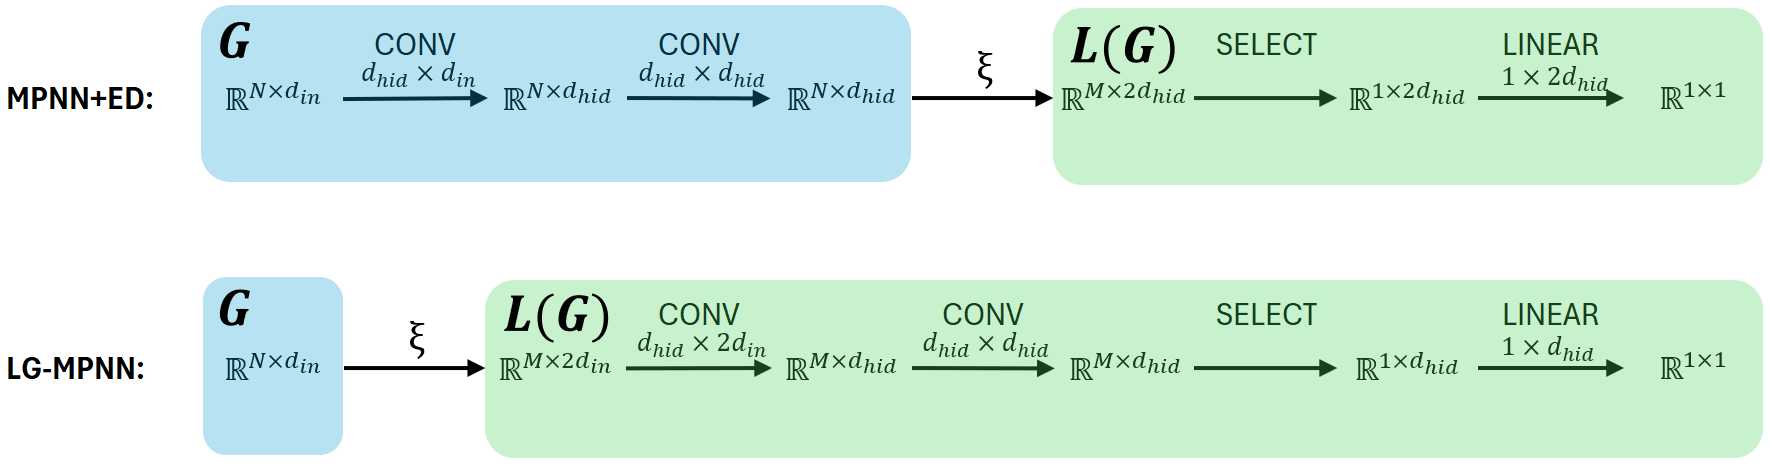
\includegraphics[width=\textwidth]{figures/architectures.PNG}
    \caption{The models used in this experiment}
    \label{fig:architectures}
\end{figure}


\paragraph{Architecture} The two models we will compare are instances of an MPNN with an edge decoder (MPNN+ED) and of an LG-MPNN, respectively. Their concrete architectures are visualized in Figure \ref{fig:architectures}.
Both models use a function $\xi$ that transforms node features on $G$ to node features on $L(G)$ by concatenating the features of both endpoints. This is not permuation invariant to the order of the endpoints, but we expect the models to learn this invariance.
During inference, both models start from the input features on a graph $G$.
The MPNN+ED model first performs two convolutions on $G$, then applies $\xi$ to compute edge features and finally selects the target link and applies a linear layer to predict the link existence.
The LG-MPNN model first applies $\xi$, then performs two convolutions on $L(G)$ and finally selects the target link and applies a linear layer to predict the link existence.
Note that the LG-MPNN model has slightly more learnable parameters than the MPNN+ED model, because the first convolutional layer has twice the number of input features.


\begin{wraptable}{r}{0.34\textwidth}
    \centering
    \small
    \caption{Hyperparameters}   \label{table:hyperparameters}
    \begin{tabular}{l l}
        \toprule
        \textbf{Hyperparameter} & \textbf{Value} \\
        \midrule
        Objective & BCE Loss \\
        Optimizer & Adam \\
        Learning Rate & $5\cdot10^{-3}$ \\
        Epochs & $80$ \\
        Batch Size & $50$ \\
        \# Convolutions & $2$ \\
        Hidden Dimension & $20/52$ \\
        Nonlinearity & ReLU \\
        \bottomrule
    \end{tabular}
\end{wraptable}


\paragraph{Hyperparameters and metrics} The hyperparameters for this experiment are summarized in Table \ref{table:hyperparameters}. Most of these were taken from the implementation of \cite{cai2021line}, but we use only 80 epochs as experiments showed that this was sufficient for convergence. We examine three setups: the Twitch dataset with $d_{hid}=20$ and the PPI dataset with $d_{hid}\in\set{20,52}$.
We evaluate the models in terms of test accuracy and test AUC, which are standard metrics for binary classification tasks. The test performance quantifies how well the model was able to capture the underlying function in the dataset. Further, we report the training accuracy and AUC to give an indication of the capacity of the model. Finally, we measure the runtime of the models to give a (relative) indication of their efficiency.


\begin{table}[ht]
    \centering
    \caption{Experimental Results}
    \label{tab:results}
    \begin{tabular}{ccccccc}
        \textbf{Experiment} & \textbf{Model} & \textbf{Test Acc} & \textbf{Test AUC} & \textbf{Train Acc} & \textbf{Train AUC} & \textbf{Runtime} \\
        \hline
        \multirow{2}{*}{\shortstack{TwitchEN \\ {\scriptsize $d_{hid}=20$}}}
        & MPNN+ED & $91.3$ & $93.8$ & $100.0$ & $99.8$ & $23.1\text{min}$ \\
        & LG-MPNN & $91.0$ & $81.9$ & $99.9$ & $88.3$ & $105.1\text{min}$ \\
        \hline
        \multirow{2}{*}{\shortstack{PPI \\ {\scriptsize $d_{hid}=20$}}}
        & MPNN+ED & $79.7$ & $85.2$ & $93.2$ & $98.5$ & $42.1\text{min}$ \\
        & LG-MPNN & $75.8$ & $80.0$ & $96.6$ & $99.3$ & $85.7\text{min}$ \\
        \hline
        \multirow{2}{*}{\shortstack{PPI \\ {\scriptsize $d_{hid}=52$}}}
        & MPNN+ED & $75.4$ & $77.4$ & $100.0$ & $99.3$ & $37.6\text{min}$ \\    
        % 1.17h for full training
        & LG-MPNN & $75.0$ & $77.5$ & $99.6$ & $98.4$ & $96.3\text{min}$ \\
        % 3.03h for full training
        \hline
    \end{tabular}
\end{table}

The results are displayed in Table \ref{tab:results}. They show a slightly better test performance for MPNN+ED compared to LG-MPNN despite its slightly smaller number of parameters. This would confirm our hypothesis that MPNN+ED is more expressive, although the difference is not very significant and further work is thus required to reach more conclusive results.
Further, the training performance is near-perfect for both models, indicating that the models both have sufficient capacity to learn the underlying function. Because of this fact, the difference is not significant enough to draw any conclusions about the relative capacity of the models.
Finally, the runtime of the LG-MPNN is consistently higher than that of the MPNN+ED, which is due to the considerably larger size of the line graph compared to the original graph. For instance, in PPI the average line graph has 1572 nodes and 59900 edges, compared to 92 nodes and 1572 edges for the original graph.
Given the similar performance for both models, the theoretical results from section \ref{sec:theory} that guarantee the higher expressiveness of MPNN+ED and the higher efficiency of MPNN+ED, we conclude that -- at least in this setting with a simple, node-attributed graph -- MPNN+ED is the better choice for the link prediction task.


\section{Outlook and Conclusion}

% Extend to edge-attributed graphs
% Extend to directed graphs
% Extend to higher-order lemmas
% Extend to knowledge graphs

% Experiment to evaluate power in terms of graph distinguishability, like in the very recent paper `The expressive power of pooling in Graph Neural Networks' with their synthetic EXPWL1 dataset, that consists of pairs of non-isomorphic graphs distinguishable by the WL-test.

In this paper, we have introduced two new variations of the Weisfeiler-Leman test tailored to edge colourings: the Line Weisfeiler-Leman Test ($\lwl$) and the Weisfeiler-Leman Test with Edge Decoding ($\wledge$).
We have theoretically characterized the power for graph distinguishability of LG-MPNN, $\lwl$, $\wledge$ and the standard WL-test, providing both an upper and a lower bound on the expressivity of LG-MPNNs and placing them in the $k$-WL hierarchy.
%
Finally, we have empirically compared the expressiveness of MPNNs with an edge decoder to that of LG-MPNNs in terms of their ability to approximate functions for the task of link prediction. Our results indicate that our hypothesis -- that MPNNs with an edge decoder are more expressive than LG-MPNNs -- is likely correct, but the results are not significant enought to draw definite conclusions.

To obtain more conclusive results, the experiment in our paper should be extended to a harder and larger link prediction task, such that the influence of the model's capacity and generalization ability becomes more apperent from the training and test performance, respectively. Further, the experiment should be repeated on more and larger datasets to ensure the results are not dataset-specific. Finally, the discrepancy between the number of learnable parameters in the two models should be eliminated to nullify its influence on the results. This can be done by modifying the architecture, which was not done in this work because we did not have the computational resources to train deeper models.

The theoretical framework proposed in this paper can be a stepping stone for further research in several directions.
First, new variations of the WL-test could be devised tailored to edge-attributed graphs, directed graphs and knowledge graphs, which can all be related to each other and the existing graph isomorphism tests in the literature.
Second, the impact of different node features on the expressiveness of LG-MPNNs and MPNNs with an edge decoder could be studied, as has been done for normal MPNNs \cite{sato2021random,feldman2022weisfeiler}.
Finally, the theoretical results could be further validated in practice by an alternative experiment that directly evaluates the power of the models in terms of graph distinguishability. This recent paper \cite{bianchi2024expressive}, for instance, uses a synthetic dataset consisting of pairs of non-isomorphic graphs distinguishable by the WL-test. The same dataset could be applied to empirically study the expressivity of LG-MPNNs and MPNNs with an edge decoder, in terms of graph distinguishability.




\appendix
\section{Proof of Theorem \ref{thm:lwl-less-than-wledge}}   \label{app:proof-lwl-less-than-wledge}

The proof of this theorem consists of two parts. In Lemma \ref{lemma:lwl-less-than-wledge} we show that $\lwl$ is less expressive than $\wledge$, and in Lemma \ref{lemma:lwl-strictly-less-than-wledge} we show that this difference is strict.

\begin{lemma}   \label{lemma:lwl-less-than-wledge}
    The $\lwl$-test is less expressive than the $\wledge$-test.
\end{lemma}

\begin{proof}
    First, we prove the following by induction on $t$. For any graph $G$ and $t\in\mbn$:
    \begin{equation}    \label{eq:wledge-refinement-of-lwl-induction-hypothesis}
        \wledge\iter{t}(G) \preceq \lwl\iter{t}(G)
    \end{equation}
    Fix the graph $G$ and shorten the notation $\wl\iter{t} \coloneq \wl\iter{t}(G)$ for clarity (and analogous for $\lwl$ and $\wledge$). The base case $t=0$ is trivially true, because the initial edge colourings of $\wledge$ and $\lwl$ are the same. For the induction step, assume (\ref{eq:wledge-refinement-of-lwl-induction-hypothesis}) holds for $t$. Then take any $uv, xy \in L(G)$ for which $\wledge\iter{t+1}(uv) = \wledge\iter{t+1}(xy)$. Due to the injectivity of $\hash$ and the decoders $\dec$, the following implications hold:
\begin{align*}
        &\wledge\iter{t+1}(uv) = \wledge\iter{t+1}(xy)
        \\
        &\RightarrowAsWideAsWLOGArrow
        \set{\wl\iter{t+1}(u),\wl\iter{t+1}(v)} = \set{\wl\iter{t+1}(x),\wl\iter{t+1}(y)}
        \\
        &\makebox[\WLOGarrowwidth][c]{$\stackrel{\text{WLOG}}{\Rightarrow}$}
        \enspace \wl\iter{t+1}(u) = \wl\iter{t+1}(x) \wedge \wl\iter{t+1}(v) = \wl\iter{t+1}(y)
        \\
        &\RightarrowAsWideAsWLOGArrow
        \begin{cases}
            \wl\iter{t}(u) = \wl\iter{t}(x) \wedge \multiset{\wl\iter{t}(d_u) \mid d_u \in \nbh(u)} = \multiset{\wl\iter{t}(d_x) \mid d_x \in \nbh(x)} \\
            \wl\iter{t}(v) = \wl\iter{t}(y) \wedge \multiset{\wl\iter{t}(d_v) \mid d_v \in \nbh(v)} = \multiset{\wl\iter{t}(d_y) \mid d_y \in \nbh(y)}
        \end{cases}
        \\
        &\RightarrowAsWideAsWLOGArrow 
        \begin{cases}
            \wledge\iter{t}(uv) = \wledge\iter{t}(xy) \\
            \multiset{\wledge\iter{t}(ud_u) \mid d_u \in \nbh(u)} = \multiset{\wledge\iter{t}(xd_x) \mid d_x \in \nbh(x)} \\
            \multiset{\wledge\iter{t}(vd_v) \mid d_v \in \nbh(v)} = \multiset{\wledge\iter{t}(yd_y) \mid d_y \in \nbh(y)}
        \end{cases}
        \\
        &\makebox[\WLOGarrowwidth][c]{$\stackrel{(\ref{eq:wledge-refinement-of-lwl-induction-hypothesis})}{\Rightarrow}$}
        \begin{cases}
            \lwl\iter{t}(uv) = \lwl\iter{t}(xy) \\
            \multiset{\lwl\iter{t}(ud_u) \mid d_u \in \nbh(u)} = \multiset{\lwl\iter{t}(xd_x) \mid d_x \in \nbh(x)} \\
            \multiset{\lwl\iter{t}(vd_v) \mid d_v \in \nbh(v)} = \multiset{\lwl\iter{t}(yd_y) \mid d_y \in \nbh(y)}
        \end{cases}
        \\
        &\RightarrowAsWideAsWLOGArrow
        \lwl\iter{t+1}(uv) = \lwl\iter{t+1}(xy)
    \end{align*}
    We have shown that $\wledge\iter{t+1}(G) \preceq \lwl\iter{t+1}(G)$, which concludes the induction step.
    Because both $\lwl$ and $\wl$ are union-preserving, it follows from Lemma \ref{lemma:refinement-distinguishability} that $\lwl$ is less expressive than $\wledge$.
\end{proof}


\begin{lemma}   \label{lemma:lwl-strictly-less-than-wledge}
    There exist graphs $G_1$ and $G_2$ that are distinguishable by $\wledge$ but not by $\lwl$.
\end{lemma}

\begin{proof}
    \begin{figure}[ht]
        \centering
        \begin{subfigure}[b]{0.25\textwidth}
            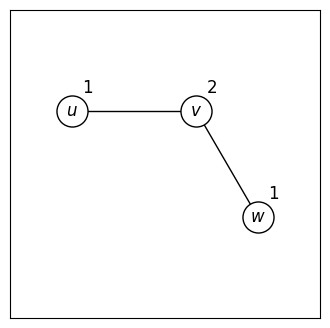
\includegraphics[width=\textwidth]{figures/lwl vs wl-ed/G1.png}
            \caption{$G_1$}
        \end{subfigure}
        \begin{subfigure}[b]{0.25\textwidth}
            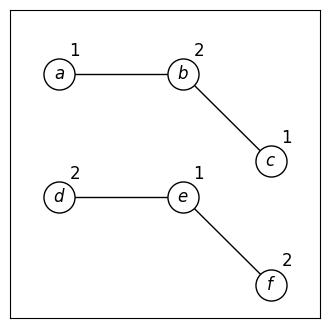
\includegraphics[width=\textwidth]{figures/lwl vs wl-ed/G2.png}
            \caption{$G_2$}
        \end{subfigure}
        \begin{subfigure}[b]{0.25\textwidth}
            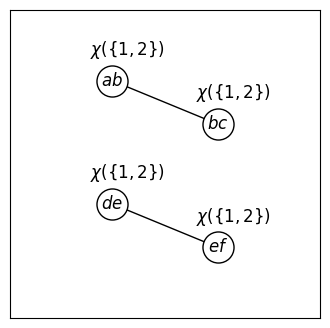
\includegraphics[width=\textwidth]{figures/lwl vs wl-ed/L(G1)-L(G2).png}
            \caption{$L(G_1)=L(G_2)$}
        \end{subfigure}
        \caption{Example of graphs $G_1$, $G_2$ that can be distinguished by $\wledge$ but not by $\lwl$.}
        \label{fig:lwl-wledge-counterexample}
    \end{figure}

    Consider the graphs $G_1$ and $G_2$ depicted in Figure \ref{fig:lwl-wledge-counterexample}.
    $\wledge$ can distinguish between these graphs. To see this, note that the colour $\wl\iter{1}(G_2)(e)$ does not occur anywhere in $\wl\iter{1}(G_1)$, so clearly $\wledge\iter{1}(G_2)(de) \notin \set{\wledge\iter{1}(G_1)(uv) \mid uv\in V(L(G_1))}$.
    In contast, $\lwl$ can never distinguish between $G_1$ and $G_2$, as their line graphs are identical. We conclude that $\lwl$ is strictly less expressive than $\wledge$.
\end{proof}


\section{Proof of Theorem \ref{thm:wledge-equal-to-wl}}   \label{app:proof-wledge-equal-to-wl}

% TODO: say something about injectivity, inverses and the computability thereof

First, we show that the multiset of node labels generated by $\wl$ uniquely determines the multiset of line graph node labels generated by $\wledge$ (Lemma \ref{lemma:wl-determines-wledge}) and vice versa (\ref{lemma:wledge-determines-wl}). Afterwards, we show how this implies Theorem \ref{thm:wledge-equal-to-wl}. Our proofs build on the injectivity of $\hash$ and $\dec$. The proofs are not constructive, but can be made so if the inverses of $\hash$ and $\dec$ on their codomains are known.

\begin{lemma}   \label{lemma:wl-determines-wledge}
    For any graph $G$, $\multiset{\wl\iter{t+1}(u) \mid u\in G}$ uniquely determines $\multiset{\wledge\iter{t}(uv) \mid uv\in L(G)}$.
\end{lemma}
\begin{proof}
    Due to the injectivity of $\hash$,
    $\multiset{\wl\iter{t+1}(u) \mid u\in G}$
    uniquely determines
    $\multiset{\left(
        \wl\iter{t}(u),
        \multiset{\wl\iter{t}(v) \mid v\in \nbh(u)}
    \right) \mid u\in G}$.

    By iterating over $u\in V(G), v\in\nbh(u)$ and collecting the sets $\set{\wl\iter{t}(u), \wl\iter{t}(v)}$, one uniquely obtains $\multiset{\set{\wl\iter{t}(u), \wl\iter{t}(v)} \mid u\in G, v\in\nbh(u)}$.
    On the other hand, note that the previous iteration goes over every edge exactly twice. Undoubling the elements yields $\multiset{\set{\wl\iter{t}(u), \wl\iter{t}(v)} \mid (u,v)\in E(G)}$, which in turn uniquely determines $\multiset{\wledge\iter{t}(uv) \mid uv\in L(G)}$.

\end{proof}

\begin{lemma}   \label{lemma:wledge-determines-wl}
    For any graph $G$, $\multiset{\wledge\iter{t}(G)(uv) \mid uv\in L(G)}$ uniquely determines $\multiset{\wl\iter{t}(u) \mid u\in G}$.
\end{lemma}
\begin{proof}
    Due to the injectivity of $\dec$,
    $\multiset{\wledge\iter{t}(uv) \mid uv\in L(G)}$
    uniquely determines
    $\multiset{\set{\wl\iter{t}(u), \wl\iter{t}(v)} \mid (u,v)\in E(G)}$.

    When `unrolling' this multiset -- i.e. creating a multiset that contains both $x$ and $y$ for each $\set{x,y}$ in the original multiset -- we deterministically obtain the multiset that contains $\wl\iter{t}(u)$ exactly $\deg(u)$ times for each $u\in G$.

    By the injectivity of $\hash$ and $t>0$, $\wl\iter{t}(u)$ uniquely determines $\deg(u) = \left\lvert\multiset{\wl\iter{t-1}(v) \mid v\in \nbh(u)}\right\rvert$ for each $u\in G$. So, if we divide the number of occurences of $\wl\iter{t}(u)$ in the unrolled multiset by $\deg(u)$ for each $u$, we deterministically obtain $\multiset{\wl\iter{t}(u) \mid u\in G}$.
\end{proof}


\begingroup
\def\thetheorem{\ref{thm:wledge-equal-to-wl}}
\begin{theorem}[restated]
    The $\wledge$-test is equally expressive as the standard WL-test.
\end{theorem}
\addtocounter{theorem}{-1}
\endgroup

\begin{proof}
    Suppose that $\wl$ cannot distinguish between $G_1$ and $G_2$, which implies $\multiset{\wl\iter{t+1}(u) \mid u\in G_1} = \multiset{\wl\iter{t+1}(u) \mid u\in G_2}$ for each $t$.
    Then it follows from Lemma \ref{lemma:wl-determines-wledge} that $\multiset{\wledge\iter{t}(uv) \mid uv\in L(G_1)} = \multiset{\wledge\iter{t}(uv) \mid uv\in L(G_2)}$ as well, and hence that $\wledge$ cannot distinguish between $G_1$ and $G_2$ either.

    Similarly, suppose that $\wledge$ cannot distinguish between $G_1$ and $G_2$, which implies $\multiset{\wledge\iter{t}(uv) \mid uv\in L(G_1)} = \multiset{\wledge\iter{t}(uv) \mid uv\in L(G_2)}$ for each $t>0$.
    Then it follows from Lemma \ref{lemma:wledge-determines-wl} that $\multiset{\wl\iter{t}(u) \mid u\in G_1} = \multiset{\wl\iter{t}(u) \mid u\in G_2}$ as well for each $t>0$, and hence that $\wl$ cannot distinguish between $G_1$ and $G_2$ either.
\end{proof}


% \begin{equation}
%     \begin{split}
%         &\multiset{\wl\iter{t+1}(u) \mid u\in G_1} = \multiset{\wl\iter{t+1}(u) \mid u\in G_2}
%         \\
%         &\Rightarrow
%         \begin{split}
%             \multiset{\left(
%                 \wl\iter{t}(u),
%                 \multiset{\wl\iter{t}(v) \mid v\in \nbh(u)}
%             \right)}_{u\in G_1}
%             =
%             \multiset{\left(
%                 \wl\iter{t}(u),
%                 \multiset{\wl\iter{t}(v) \mid v\in \nbh(u)}
%             \right)}_{u\in G_2}
%         \end{split}
%     \end{split}
% \end{equation}
% When iterating over all pairs $(u,v)$ with $u\in V(G_i), v\in\nbh(u)$ and collecting the sets $\set{\wl\iter{t}(u), \wl\iter{t}(v)}$ in a multiset, the previous equation implies that the result will be the same for $i\in\set{1,2}$:
% \begin{equation}
%     \multiset{\set{\wl\iter{t}(u), \wl\iter{t}(v)} \mid u\in V(G_1), v\in \nbh(u)} = \multiset{\set{\wl\iter{t}(u), \wl\iter{t}(v)} \mid u\in V(G_2), v\in \nbh(u)}
% \end{equation}
% On the other hand, note that the previously described iteration goes over every edge $(u,v)\in E(G_i)$ exactly twice, so the multisets in the previous equation contain $\set{\wl\iter{t}(u), \wl\iter{t}(v)}$ twice for each edge $(u,v)\in E(G_i)$. Undoubling the elements yields:
% \begin{equation}
%     \begin{split}
%         &\multiset{\set{\wl\iter{t}(u), \wl\iter{t}(v)} \mid (u,v)\in E(G_1)}
%         =
%         \multiset{\set{\wl\iter{t}(u), \wl\iter{t}(v)} \mid (u,v)\in E(G_2)}
%         \\
%         &\Rightarrow
%         \multiset{\wledge\iter{t}(uv) \mid uv\in L(G_1)}
%         =
%         \multiset{\wledge\iter{t}(uv) \mid uv\in L(G_2)}
%     \end{split}
% \end{equation}
% From which follows that $\wledge$ cannot distinguish $G_1$ and $G_2$ either. We conclude that $\wledge$ is at most as expressive as $\wl$.


\bibliographystyle{unsrt}
\bibliography{refs}


\end{document}